\documentclass[12pt,a4paper]{report}

% ============================================
% PACKAGES
% ============================================
\usepackage[margin=1in]{geometry}           % Page margins
\usepackage{graphicx}                       % For including images
\usepackage[inkscapeformat=pdf]{svg}        % SVG support with Inkscape
\usepackage{setspace}                       % Line spacing
\usepackage{titlesec}                       % Chapter/section formatting
\usepackage{tocloft}                        % Table of contents formatting
\usepackage{mathptmx}                       % Times-like font
\usepackage[utf8]{inputenc}                 % UTF-8 encoding
\usepackage{hyperref}                       % Clickable links in TOC
\usepackage{caption}                        % Figure captions
\usepackage{enumitem}                       % Better list formatting
\usepackage{ragged2e}                       % Better text justification

% ============================================
% FORMATTING SETTINGS
% ============================================
\onehalfspacing                             % 1.5 line spacing
\justifying                                 % Full text justification

% Chapter formatting (without chapter numbers)
\titleformat{\chapter}[display]
  {\normalfont\huge\bfseries}{}{0pt}{\Huge}
\titlespacing*{\chapter}{0pt}{0pt}{40pt}

% Section formatting
\titleformat{\section}
  {\normalfont\Large\bfseries}{\thesection}{1em}{}
\titleformat{\subsection}
  {\normalfont\large\bfseries}{\thesubsection}{1em}{}

% Hyperref settings
\hypersetup{
    colorlinks=true,
    linkcolor=black,
    urlcolor=blue,
    citecolor=black
}

% ============================================
% DOCUMENT BEGINS
% ============================================
\begin{document}

% ============================================
% FRONT MATTER (Roman numerals)
% ============================================
\pagenumbering{gobble}  % Suppress page numbering for title page

% --------------------------------------------
% TITLE PAGE
% --------------------------------------------
\begin{titlepage}
    \centering

    \vspace*{1cm}

    
\includegraphics[width=3cm]{nitm_logo.png}

    \vspace{1.5cm}

    {\LARGE\bfseries Report}

    \vspace{1cm}

    {\Large On}

    \vspace{0.5cm}

    {\LARGE\bfseries CS603 - Internship Work}

    \vspace{1cm}

    {\Large At}

    \vspace{0.5cm}

    {\LARGE\bfseries Pamir AI}

    \vspace{0.3cm}

    {\large Marina Blvd, San Francisco, CA, 94123-1284, United States}

    \vspace{1.5cm}

    {\large Submitted in partial fulfillment of the requirements}

    {\large for the award of the degree of}

    \vspace{0.5cm}

    {\Large\bfseries Master of Computer Science and Engineering}

    \vspace{1cm}

    {\large by}

    \vspace{0.5cm}

    {\Large\bfseries Utsav Balar}

    {\large Roll No: T24CS003}

    \vfill

    {\large\bfseries Department of Computer Science and Engineering}

    {\large\bfseries National Institute of Technology, Meghalaya}

    {\large Sohra, Cherrapunji -- 793108}

    \vspace{0.5cm}

    {\large\bfseries 2025}

\end{titlepage}

\pagenumbering{roman}  % Start roman numbering from certificate pages

% --------------------------------------------
% CERTIFICATE FROM THE COMPANY
% --------------------------------------------
\newpage
\chapter*{Certificate from the Company}
\addcontentsline{toc}{chapter}{Certificate from the Company}

\vspace{1cm}

This is to certify that \textbf{Utsav Balar}, Roll No. \textbf{T24CS003}, student of Master of Computer Science and Engineering at National Institute of Technology, Meghalaya, has been working as a full-time intern at \textbf{Pamir AI} since \textbf{31st May 2025} and is currently continuing with the company.

\vspace{0.5cm}

During this ongoing internship, he has worked on various projects related to Linux kernel development, BSP engineering, and edge AI hardware integration. His work includes developing custom kernel drivers, creating software development kits, and implementing system services for our Distiller product line.

\vspace{0.5cm}

He has shown excellent technical skills, dedication, and commitment throughout this long-term internship. His contributions have been valuable to our product development efforts.

\vspace{0.5cm}

We wish him all the best for his future endeavors.

\vspace{2cm}

\noindent
\textbf{Tianqi Ye} \\
Co-founder and CTO \\
Pamir AI

\vspace{1.5cm}

\noindent
\textbf{Signature:} \underline{\hspace{2cm}\textit{Tianqi Ye}\hspace{2cm}}

\vspace{0.5cm}

\noindent
\textbf{Date:} \underline{\hspace{1cm}27/10/2025\hspace{1cm}} \hspace{1cm} \textbf{Place:} \underline{\hspace{1cm}San Francisco, CA\hspace{1cm}}

% --------------------------------------------
% CERTIFICATE FROM THE INSTITUTE
% --------------------------------------------
% \newpage
% \chapter*{Certificate from the Institute}
% \addcontentsline{toc}{chapter}{Certificate from the Institute}
%
% \vspace{1cm}
%
% This is to certify that the report entitled \textbf{``Edge AI Hardware and Software Development''} submitted by \textbf{Utsav Balar}, Roll No. \textbf{T24CS003}, is a record of bonafide work carried out by him under my supervision and guidance in partial fulfillment of the requirements for the award of the degree of \textbf{Master of Computer Science and Engineering} from the \textbf{Department of Computer Science and Engineering, National Institute of Technology, Meghalaya}.
%
% \vspace{2cm}
%
% \noindent
% \textbf{Dr. Ngangbam Herojit Singh} \\
% Faculty Supervisor \\
% Department of Computer Science and Engineering \\
% National Institute of Technology, Meghalaya
%
% \vspace{1.5cm}
%
% \noindent
% \textbf{Signature:} \underline{\hspace{6cm}}
%
% \vspace{0.5cm}
%
% \noindent
% \textbf{Date:} \underline{\hspace{4cm}} \hspace{1cm} \textbf{Place:} \underline{\hspace{4cm}}

% --------------------------------------------
% ACKNOWLEDGEMENT
% --------------------------------------------
\newpage
\chapter*{Acknowledgement}
\addcontentsline{toc}{chapter}{Acknowledgement}

\vspace{1cm}

I would like to express my sincere gratitude to all those who supported me during my internship at Pamir AI.

\vspace{0.5cm}

First and foremost, I am grateful to \textbf{Tianqi Ye} and \textbf{Kevin Zhang}, the co-founders of Pamir AI, for giving me this opportunity and for their constant guidance throughout the internship. Their expertise in edge AI hardware and their vision for creating accessible AI solutions inspired me greatly.

\vspace{0.5cm}

I would like to thank my academic supervisor, \textbf{Dr. Ngangbam Herojit Singh}, for his support and guidance throughout this internship period.

\vspace{0.5cm}

I am also thankful to \textbf{Nischal}, my fellow intern, for the collaborative work environment and helpful discussions we had during the internship.

\vspace{0.5cm}

I express my gratitude to the \textbf{Department of Computer Science and Engineering} at \textbf{National Institute of Technology, Meghalaya} for providing me with the opportunity to undertake this internship as part of my curriculum.

\vspace{0.5cm}

Finally, I thank my family and friends for their continuous support and encouragement throughout this journey.

\vspace{2cm}

\begin{flushright}
\textbf{Utsav Balar} \\
T24CS003
\end{flushright}

% --------------------------------------------
% ABSTRACT
% --------------------------------------------
\newpage
\chapter*{Abstract}
\addcontentsline{toc}{chapter}{Abstract}

\vspace{1cm}

I've been working remotely as a Linux Kernel and BSP Engineer at Pamir AI since May 31st, 2025. Pamir AI is a San Francisco-based startup building edge AI hardware, and I'm writing this from my desk in Surat, Gujarat, nearly six months into the internship.

\vspace{0.5cm}

My main responsibility has been developing complete Board Support Packages for the Distiller product line across three different hardware platforms: Raspberry Pi CM5, Rockchip RK3568, and RK3576 SoCs. The work involved writing custom kernel drivers for e-ink displays and audio codecs, designing the SAM (Signal Aggregation Module) protocol for microcontroller communication, developing the Distiller SDK to provide userspace APIs for hardware interaction, building a wifi provisioning service for headless devices, and the entire software ecosystem for Distiller devices.

\vspace{0.5cm}

The scope covered multiple layers of the stack. I wrote kernel drivers, debugged UART communication issues, handled Debian packaging for all the Distiller softwares, and worked on the application layer when needed. Each platform had specific quirks—particularly around GPIO numbering schemes and device tree structures—which required careful abstraction layer design to maintain a single codebase across all three SoCs.

\vspace{0.5cm}

The internship provided hands-on experience with production embedded Linux development. Working remotely meant debugging hardware issues primarily through serial console logs and careful code instrumentation rather than direct hardware access. The work also involved learning new tooling around Debian packaging (debuild, lintian) and deployment workflows specific to embedded devices.

\vspace{1cm}

\noindent
\textbf{Keywords:} Linux Kernel Development, Device Drivers, BSP Engineering, Edge AI, Embedded Systems, UART Communication, Debian Packaging

% --------------------------------------------
% TABLE OF CONTENTS
% --------------------------------------------
\newpage
\tableofcontents

% ============================================
% MAIN MATTER (Arabic numerals)
% ============================================
\newpage
\pagenumbering{arabic}

% --------------------------------------------
% CHAPTER 1: INTRODUCTION
% --------------------------------------------
\chapter{Introduction}

\section{About Pamir AI}

Pamir AI is a technology startup founded in 2024 and based in San Francisco, California. The company was founded by \textbf{Tianqi Ye} and \textbf{Kevin Zhang}, both of whom bring extensive experience from leading technology companies.

\vspace{0.3cm}

Tianqi Ye previously worked at Qualcomm Research Center, where he developed edge-side neural networks for autonomous driving and holds 2 patents under the Qualcomm Innovation Fellowship. He was also a core team member for Qualcomm's Autonomous Driving SoC Platform in their B2B business division, and has worked as a Software Development Engineer at Amazon.

\vspace{0.3cm}

Kevin Zhang comes from Microsoft's Surface team, where he was part of the core R\&D group for compute devices. He has extensive experience in consumer electronics development and has iterated through 5 generations of Surface product development.

\vspace{0.3cm}

Currently, Pamir AI is a small team of approximately 5 people, working on cutting-edge edge AI hardware and software solutions. Despite its small size, the company is making significant strides in bringing AI capabilities to compact, power-efficient devices.

\begin{figure}[htbp]
    \centering
    
\includegraphics[width=0.6\textwidth]{pamirai_logo.png}
    \caption{Pamir AI Company Logo}
\end{figure}

\section{Company Vision and Mission}

Pamir AI specializes in developing edge AI hardware and software solutions that operate without constant internet connectivity. The company's vision is to make AI accessible and practical for real-world applications where cloud connectivity is unreliable or unavailable.

\vspace{0.3cm}

The company focuses on creating compact, efficient AI-powered devices that can run complex AI models locally, without depending on cloud services. This approach is particularly valuable in scenarios where privacy, latency, or connectivity are concerns.

\section{Products and Services}

Pamir AI has developed three main products in the Distiller series:

\vspace{0.3cm}

\textbf{Distiller Alpha:} A pocket-sized Linux server that runs AI applications 24/7 with remote access capabilities via QR code. It is designed as a portable, always-on computing platform that users can carry and access remotely.

\vspace{0.3cm}

\textbf{Distiller BHV:} A compact AI hardware device created as a demonstration project for DEFCON's Bio Hacking Village conference. It showcases efficient on-device AI processing without relying on cloud connectivity. This device features a large e-ink display, custom audio codec, input buttons, LEDs, and serves as a proof-of-concept for how Pamir AI's edge AI technology can be applied to various domains, including medical and biological applications.

\vspace{0.3cm}

\textbf{Distiller Air:} An ultralightweight AI hardware device with cellular connectivity designed for remote AI applications. This represents the latest evolution in the Distiller product line, optimizing for portability and wireless connectivity.

\begin{figure}[htbp]
    \centering
    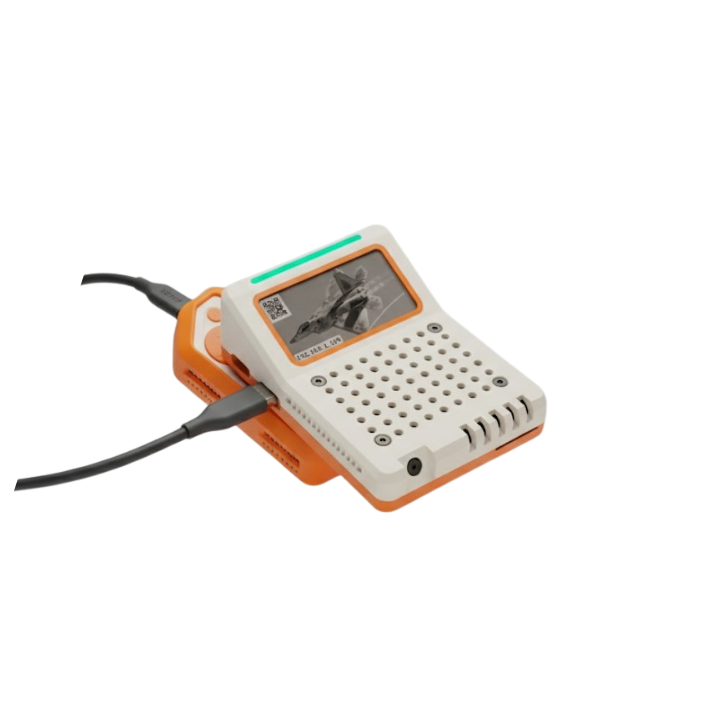
\includegraphics[width=0.7\textwidth]{distiller_alpha.png}
    \caption{Distiller Alpha - Pocket-sized Linux Server}
\end{figure}

\vspace{0.5cm}

\begin{figure}[htbp]
    \centering
    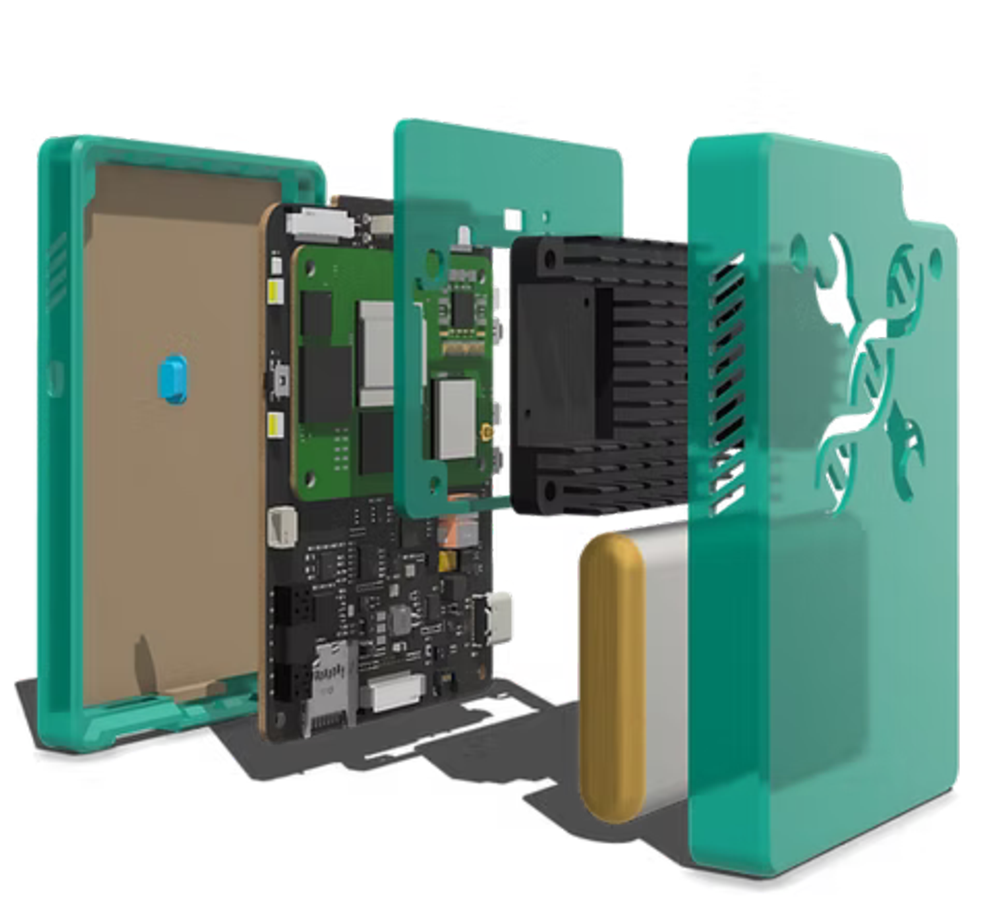
\includegraphics[width=0.7\textwidth]{distiller_bhv.pdf}
    \caption{Distiller BHV - AI Device for Bio Hacking Village}
\end{figure}

\vspace{0.5cm}

\begin{figure}[htbp]
    \centering
    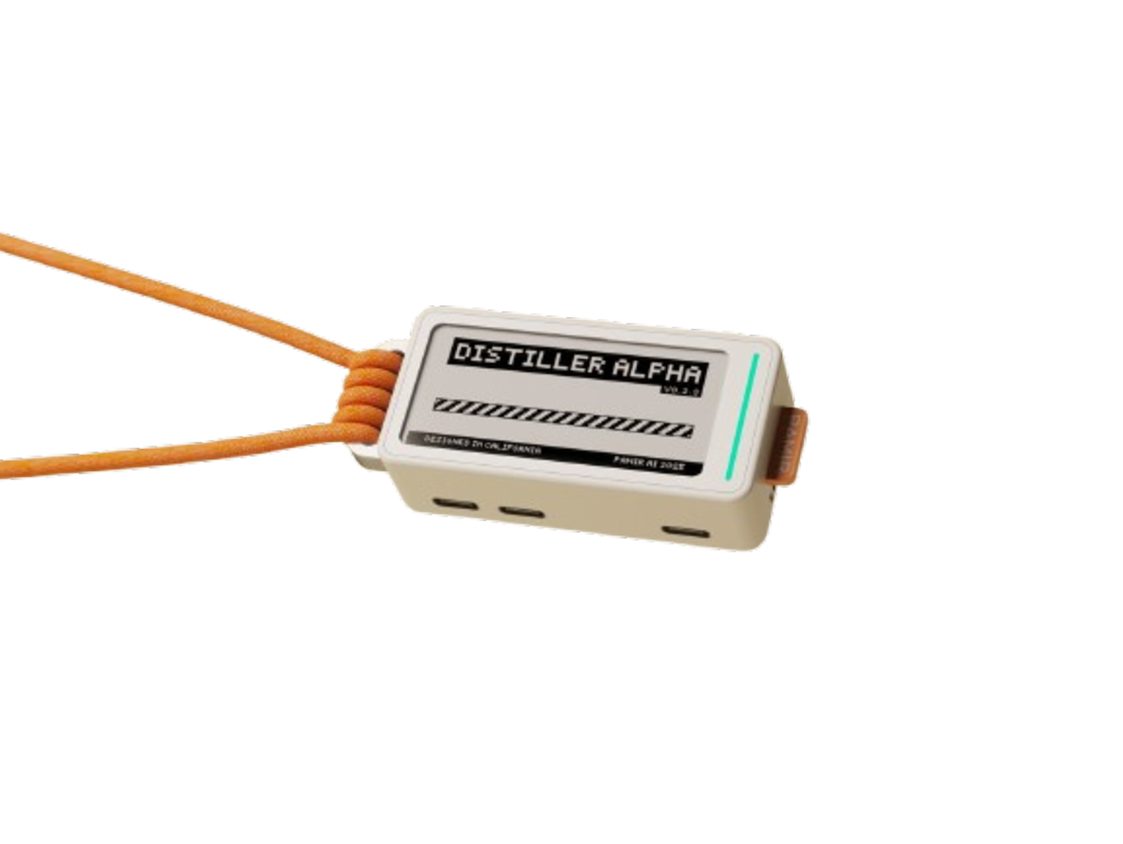
\includegraphics[width=0.7\textwidth]{distiller_air.pdf}
    \caption{Distiller Air - Ultralightweight AI Hardware with Cellular Connectivity}
\end{figure}

\section{Industry and Market Position}

Pamir AI operates in the edge AI hardware and software solutions sector, which is a rapidly growing field. The company's focus on building versatile, offline-capable AI hardware positions it uniquely in the market for applications requiring privacy, low latency, and independence from cloud connectivity.

\vspace{0.3cm}

The company has been actively involved in the AI hardware community, including presentations at industry events such as DEFCON's Bio Hacking Village, where the BHV device was demonstrated as a proof-of-concept for medical applications. Their approach of combining efficient AI models with custom hardware solutions addresses real-world problems across various sectors where reliable, private, and offline AI processing is essential.

% --------------------------------------------
% CHAPTER 2: INTERNSHIP DETAILS
% --------------------------------------------
\chapter{Internship Details}

\section{Objectives of the Internship}

The primary objectives of my internship at Pamir AI were:

\begin{enumerate}[itemsep=0.3cm]
    \item To gain better experience in Linux kernel development and device driver programming
    \item To improve upon my BSP (Board Support Package) development knowledge.
    \item To learn how to integrate custom hardware components with the Linux kernel
    \item To develop system-level software for edge AI devices
    \item To work on real-world product development in a startup environment
\end{enumerate}

\section{Duration and Mode}

This is a \textbf{long-term, full-time internship} that started on \textbf{31st May 2025} and is \textbf{currently ongoing}. As of the writing of this report in October 2025, I have been working with Pamir AI for approximately 5 months and continue to contribute to the company's projects. The internship is conducted entirely in \textbf{remote mode} due to the company being based in San Francisco, California, while I am located in Surat, Gujarat, India.

\vspace{0.3cm}

Working remotely in a full-time capacity required strong self-discipline and effective communication. I work 6-8 hours per day, coordinating with the team across different time zones. The remote nature of the work has taught me valuable lessons about asynchronous communication, independent problem-solving, and maintaining productivity without direct supervision.

\section{Role and Responsibilities}

My official designation was \textbf{Linux Kernel and BSP Engineer}. However, the nature of work in a startup meant that my responsibilities extended beyond traditional role boundaries.

\vspace{0.3cm}

My primary responsibilities included:

\begin{enumerate}[itemsep=0.3cm]
    \item \textbf{Kernel Driver Development:} Writing custom Linux kernel drivers for various hardware components including e-ink displays, audio codecs, and UART communication interfaces.

    \item \textbf{BSP Development:} Creating and maintaining board support packages for multiple hardware platforms, ensuring compatibility across different SoC architectures.

    \item \textbf{SDK Development:} Designing and implementing userspace APIs and libraries for application developers to interact with hardware components.

    \item \textbf{System Services:} Developing system-level services for device management, including wifi provisioning and device configuration.

    \item \textbf{Debian Packaging:} Creating proper Debian packages for all software components, ensuring compliance with packaging standards and easy deployment.

    \item \textbf{Testing and Documentation:} Regularly testing hardware components, debugging issues, and writing documentation for drivers and SDKs.

    \item \textbf{Build System Integration:} Working with build tools and package management systems to streamline the development and deployment process.
\end{enumerate}

\section{Mentorship and Team Structure}

I worked under the direct mentorship of both co-founders: \textbf{Tianqi Ye} (Co-founder and CTO) and \textbf{Kevin Zhang} (Co-founder and CEO). Having access to both founders provided me with unique insights into both technical and business aspects of the company.

\vspace{0.3cm}

The team structure was very flat, with only about 5 people in total. This meant I had direct communication with the leadership and my work had immediate impact on the product.

\vspace{0.3cm}

I communicated with my mentors daily through Slack, where I received code reviews and ad-hoc help whenever needed. The informal communication style of a startup made it easy to ask questions and get quick feedback.

\vspace{0.3cm}

I also worked alongside \textbf{Nischal}, another software engineer intern, which provided opportunities for collaboration and peer learning.

\vspace{0.3cm}

The company held monthly all-hands meetings where we discussed company updates, progress on various projects, and future plans. These meetings gave me visibility into the bigger picture of the company's direction.

\vspace{0.3cm}

My work was assigned through GitHub issues and verbal instructions via Slack, which gave me a good understanding of industry-standard development workflows.

% --------------------------------------------
% CHAPTER 3: WORK DONE DURING INTERNSHIP
% --------------------------------------------
\chapter{Work Done During Internship}

\section{Initial Phase: Hardware Bringup}

I'd actually been working with the Pamir AI team since March, so by the time my official internship started in late May, I was already familiar with their workflow. The first major task was bringing up the Distiller BHV hardware.

\vspace{0.3cm}

The BHV device was being built for DEFCON's Bio Hacking Village conference. It included several custom hardware components: a large e-ink display, a custom audio codec, UART communication between an RP2040 microcontroller and the Raspberry Pi CM5, input buttons, and LEDs. Most of these needed custom kernel drivers.

\vspace{0.3cm}

My job was to get each component working with the Linux kernel. This meant working through datasheets, writing drivers, and integrating with existing kernel frameworks. The device tree configuration required careful attention to register mappings and timing requirements, particularly where vendor documentation was incomplete.

\vspace{0.3cm}

The e-ink display required writing a driver from scratch—there wasn't an existing Linux driver for this particular controller. I worked through the 200-page datasheet to understand the refresh sequences and timing constraints. E-ink displays have different refresh characteristics compared to LCDs, which affected the driver implementation. My initial version produced visual artifacts (ghosting, partial refreshes, stuck pixels) because I was using refresh patterns appropriate for LCD controllers. Adjusting the timing and command sequences resolved these issues.

\vspace{0.3cm}

The audio codec integration with ALSA was more straightforward since I could reference similar drivers in the kernel tree. I wrote a machine driver to configure the codec and connect it to the audio subsystem.

\vspace{0.3cm}

The GPIO work for buttons and LEDs involved device tree configuration and standard GPIO framework calls. The device tree needed to be correct for the kernel to recognize the hardware properly.

\begin{figure}[htbp]
    \centering
    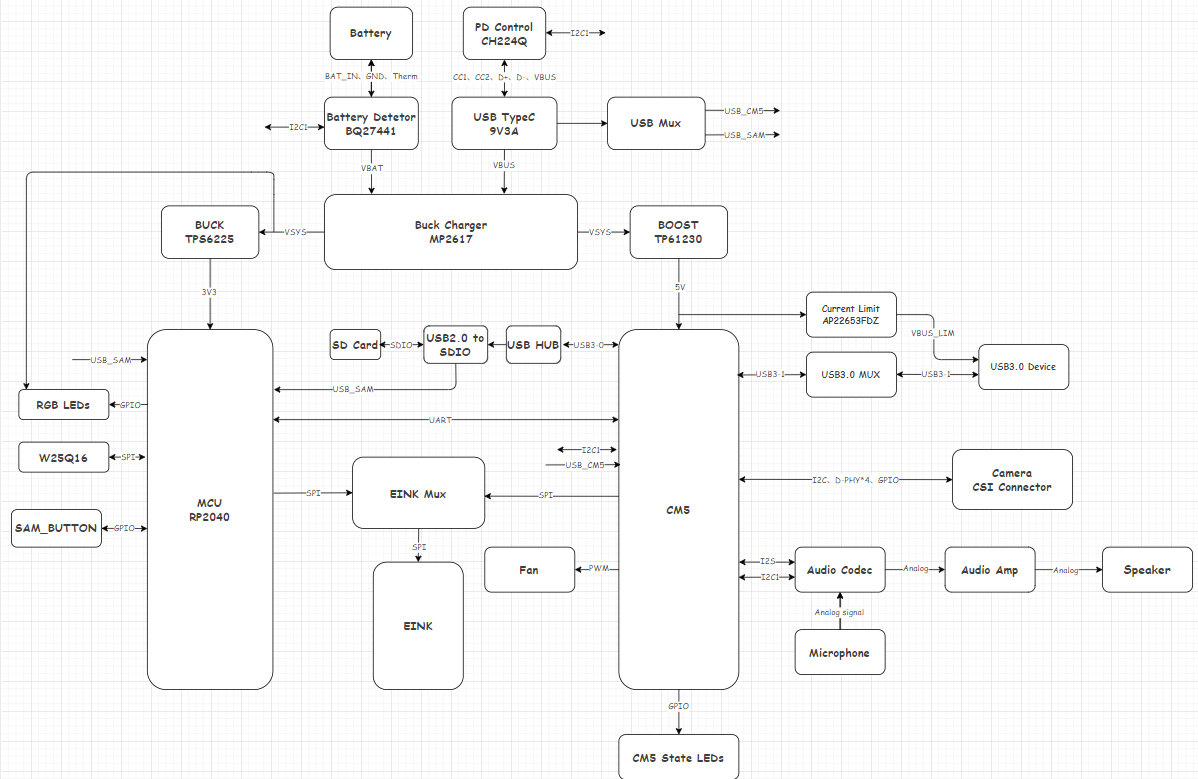
\includegraphics[width=0.8\textwidth]{bhv_hardware_architecture.png}
    \caption{Distiller BHV Hardware Architecture}
\end{figure}

\section{SAM Protocol Development}

The SAM (Signal Aggregation Module) protocol required designing a reliable UART communication scheme from scratch for the Distiller BHV device.

\vspace{0.3cm}

The challenge: the Raspberry Pi CM5 and RP2040 microcontroller needed bidirectional communication over UART with reliable delivery and no packet loss under high throughput. The design had to balance simplicity (the RP2040 is resource-constrained) with robustness (lost commands or corrupted data weren't acceptable).

\vspace{0.3cm}

I designed the entire protocol: message structure, command set, error handling, and flow control. My first approach used fixed-size packets with a simple header and checksum. This worked for basic testing but failed under load—I was getting buffer overflows on the RP2040 side when messages arrived faster than it could process them. The issue was a miscalculation in buffer sizing for the checksum field, which took about three days to identify and fix.

\vspace{0.3cm}

The second iteration added a more sophisticated flow control mechanism, but this introduced timing issues. The RP2040 would occasionally miss acknowledgment packets, triggering retransmissions that exacerbated the problem. Adjusting timing parameters helped but created edge cases elsewhere.

\vspace{0.3cm}

The final implementation used variable-length packets with a more robust framing scheme and better buffering on both sides. On the Linux side, I wrote a kernel driver that handles UART communication and exposes a clean interface for userspace. The driver processes incoming packets and manages the protocol state machine.

\vspace{0.3cm}

This work reinforced the importance of designing for real-world conditions rather than ideal test scenarios. The protocol needed to handle timing variations, packet loss, and unexpected state transitions reliably.

\begin{figure}[htbp]
    \centering
    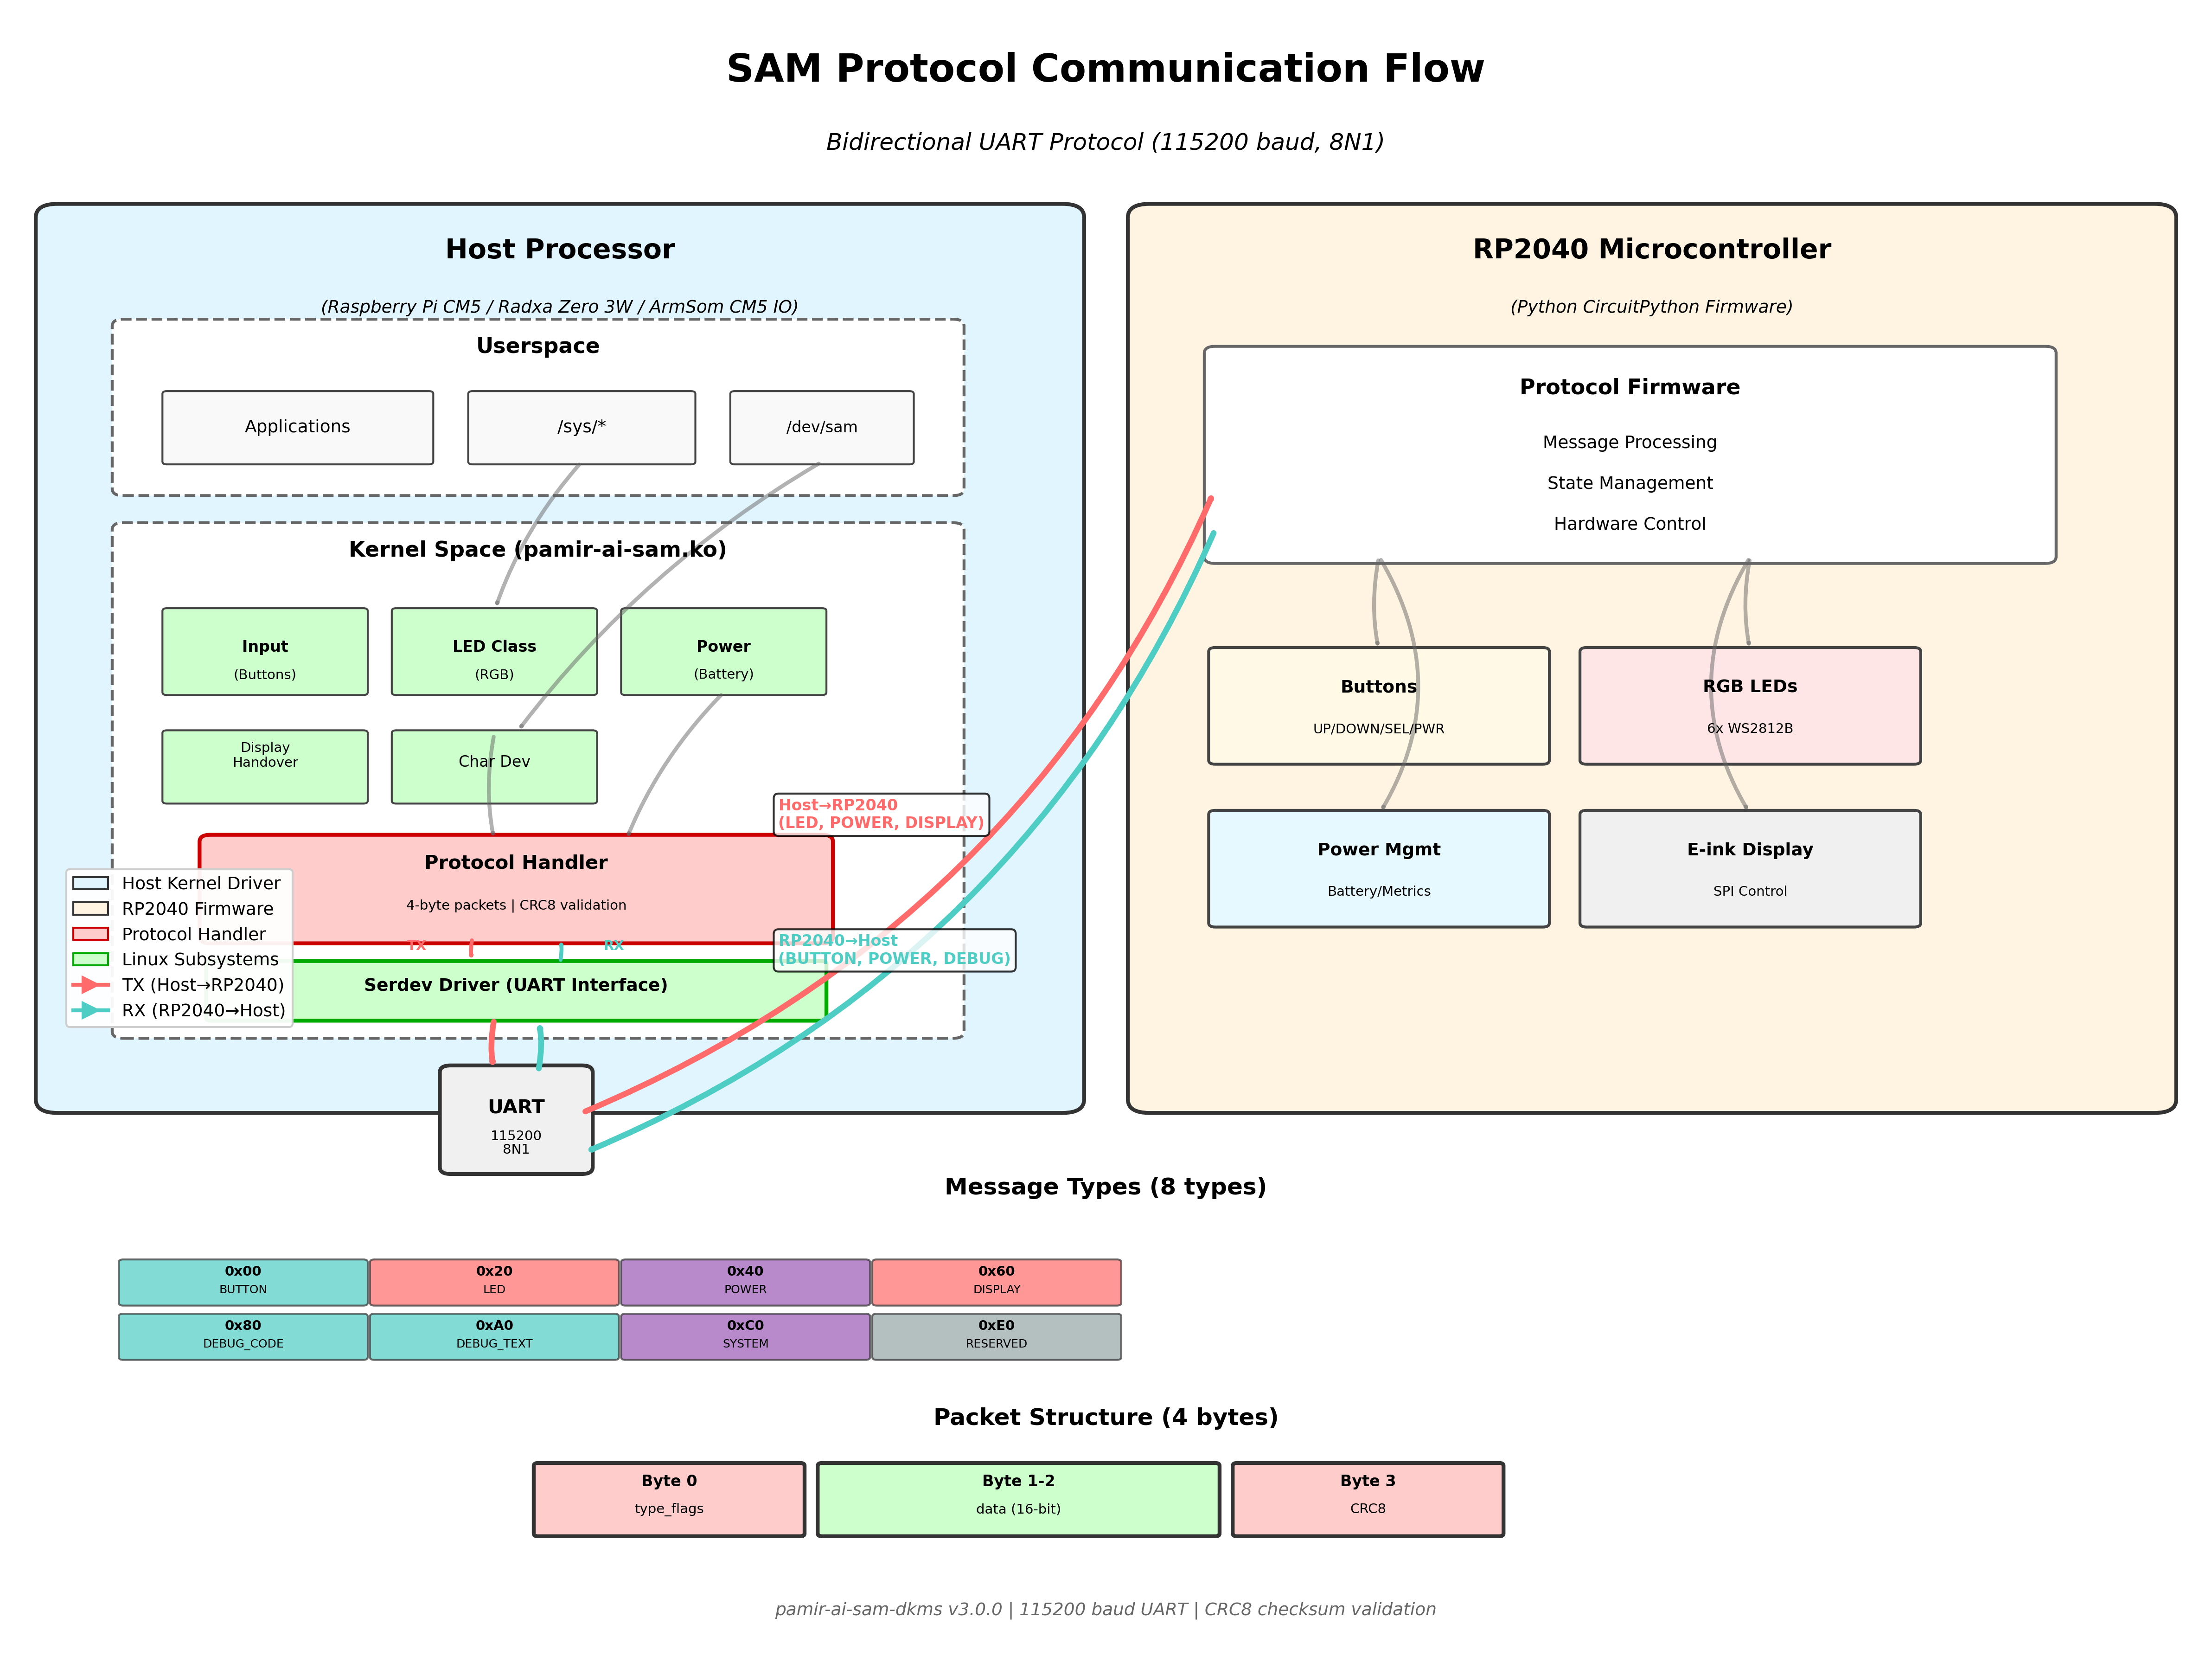
\includegraphics[width=0.7\textwidth]{sam-protocol-flow.png}
    \caption{SAM Protocol Communication Flow}
\end{figure}

\section{Distiller SDK Development}

Building the Distiller SDK meant providing application developers with clean APIs to control the hardware without requiring kernel-level knowledge. The goal was to let someone use the e-ink display or audio codec with a few Python function calls rather than understanding ALSA internals or device driver architecture.

\vspace{0.3cm}

The SDK had three main layers. First, I wrote kernel modules that exposed hardware functionality to userspace—relatively straightforward since I'd already built the underlying drivers. Then came the Python libraries that wrapped everything with clean, high-level APIs, designed to make common tasks simple while still allowing low-level control when needed.

\vspace{0.3cm}

The platform abstraction layer required the most work. We started with just the Raspberry Pi CM5, so I initially called it ``distiller-cm5-sdk'' and made CM5-specific assumptions throughout the code. When the company decided to support Rockchip RK3568 and RK3576 SoCs, I refactored everything into a platform-agnostic ``distiller-sdk.''

\vspace{0.3cm}

That refactoring took about two weeks. The challenge was handling different GPIO numbering schemes, device tree structures, and platform-specific timing differences. I found multiple places where I'd hardcoded assumptions about the CM5's hardware layout. Each platform had specific quirks—the Rockchip SoCs handled certain peripherals differently, requiring more than just swapping configuration values.

\vspace{0.3cm}

The final SDK ended up cleaner than the original. Supporting multiple platforms required more careful consideration of abstraction boundaries and API design.

\section{WiFi Provisioning Service}

Headless devices have a classic chicken-and-egg problem: how do you connect to wifi when you don't have a screen or keyboard? I'd seen solutions using Bluetooth pairing, physical buttons with LED feedback, even USB configuration modes. None of those fit our hardware constraints or user experience goals.

\vspace{0.3cm}

I built the ``distiller-services'' daemon to handle this, among other system tasks. The approach: create a temporary access point that users connect to with their phone, show them a web interface to select their home network and enter the password, then shut down the AP and connect to their actual wifi.

\vspace{0.3cm}

The state management required careful attention to edge cases. What happens if they enter the wrong password? If their network is temporarily down? If the device reboots mid-provisioning? If they walk out of range while the AP is still running?

\vspace{0.3cm}

I tested this extensively on my own router—probably fifty iterations—deliberately entering wrong passwords and unplugging things to identify failure modes. The service needed to handle these edge cases gracefully while remaining simple for non-technical users. I implemented state persistence for configurations across reboots, retry logic for temporary network issues, and clear error messages for common problems.

\vspace{0.3cm}

The web interface was intentionally minimal—just a list of available networks and a password field. I tested it on different phones to verify the captive portal detection worked correctly. Some phones refuse to show the configuration page if they detect the device has no internet connectivity, which required workarounds with DNS and HTTP responses.

\vspace{0.3cm}

The challenge was ensuring the service worked reliably across different network environments, not just on my test setup. The final implementation handled most common scenarios without requiring users to understand the underlying mechanism.

\begin{figure}[htbp]
    \centering
    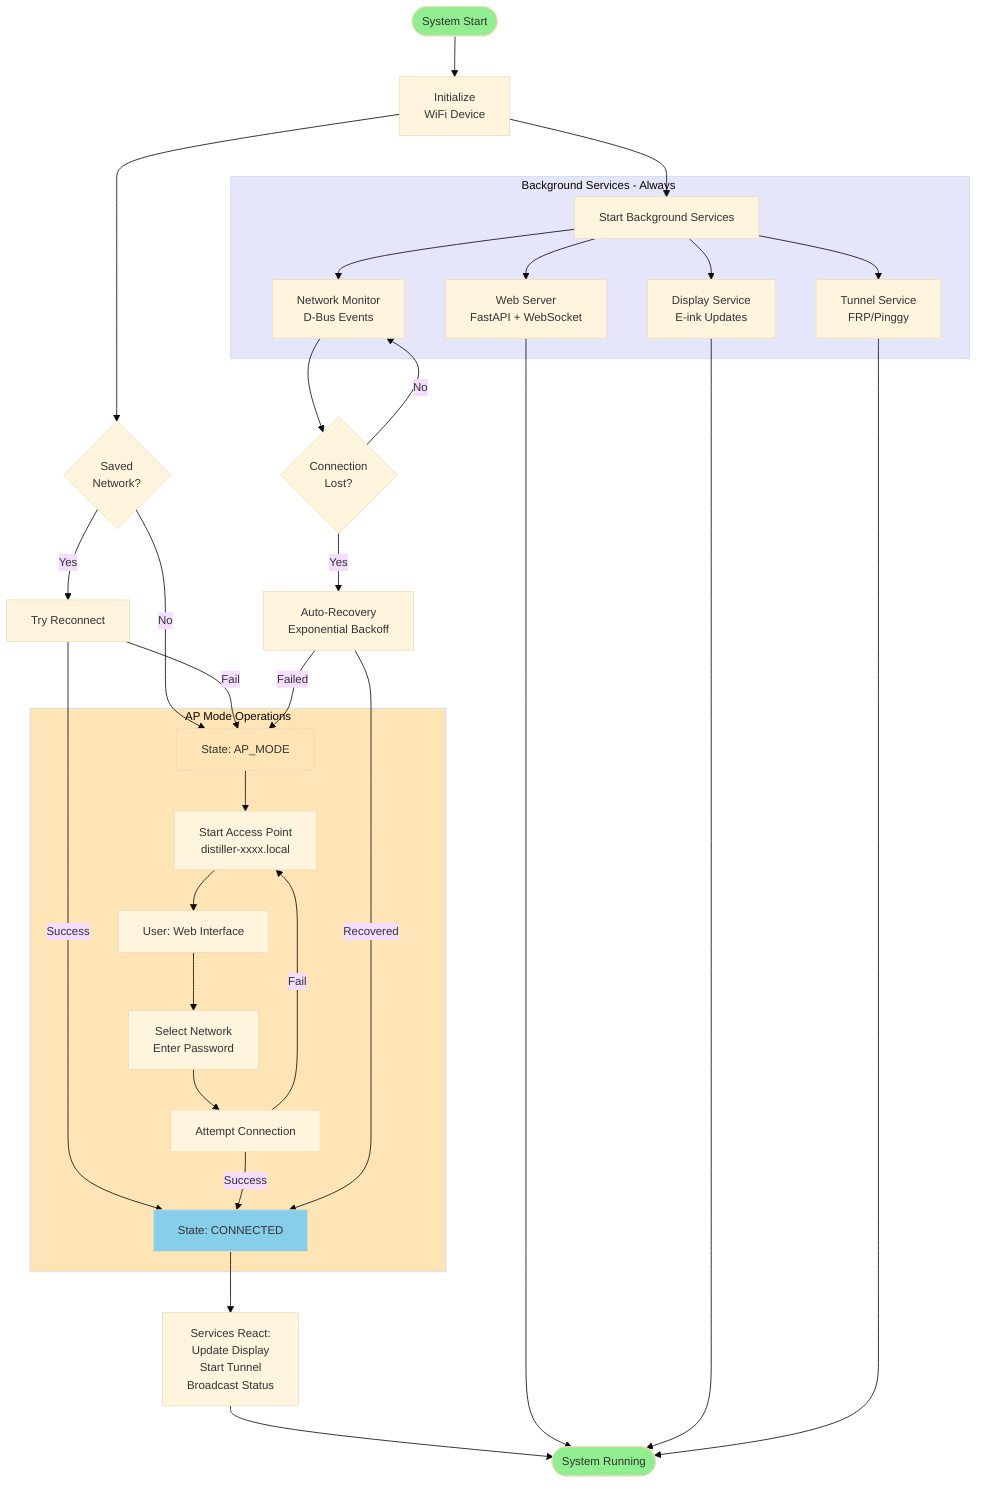
\includegraphics[width=0.8\textwidth]{wifi_provisioning_flow.png}
    \caption{WiFi Provisioning User Flow}
\end{figure}

\section{Additional Projects and Contributions}

Beyond the three major projects mentioned above, I contributed to several other initiatives:

\vspace{0.3cm}

\textbf{Distiller CM5 Python Application:} I worked on the complete demonstration application written in Python and QT for the Distiller BHV device. This application ties together all the hardware components (e-ink display, buttons, microphone) to showcase the device's AI capabilities. The application was designed for the DEFCON Bio Hacking Village presentation. Working on this gave me exposure to application-level development and how it integrates with the lower-level systems I had built.

\vspace{0.3cm}

\textbf{APT Server Integration:} I worked on integrating the Distiller device packages with an Aptly-based APT server. This involved creating proper Debian packages for all the software components and setting up the repository structure for easy installation and updates.

\vspace{0.3cm}

\textbf{APT Server CLI:} I developed a command-line interface for managing the APT server. This tool allows the team to easily manage package repositories, handle versioning, and deploy updates.

\vspace{0.3cm}

\textbf{APT Server Portal:} I created a web portal for the APT server that provides a user-friendly interface for managing packages and monitoring device deployments.

\vspace{0.3cm}

\textbf{Regular Tasks:} Throughout the internship, I regularly performed testing of hardware components, debugging issues when they arose, and writing documentation for the drivers and SDKs I developed. These routine tasks were essential for maintaining code quality and ensuring smooth product development.

\section{Technologies and Tools Used}

During the internship, I worked with a diverse set of technologies and tools:

\vspace{0.3cm}

\textbf{Programming Languages:} I primarily used C for kernel driver development, Python for userspace services and applications, and Bash for scripting. I also worked with Rust, JavaScript, TypeScript, HTML, CSS, and QML for various components of the system.

\vspace{0.3cm}

\textbf{Operating Systems:} I worked extensively with Linux, primarily Debian-based distributions. I also used MacOS for some development tasks.

\vspace{0.3cm}

\textbf{Hardware Platforms:} The main platforms I worked with were Raspberry Pi CM5 (using Broadcom BCM2712 SoC), Rockchip RK3568 and RK3576 SoCs, and the RP2040 microcontroller.

\vspace{0.3cm}

\textbf{Development Tools:} I used Neovim as my primary editor, Minicom for serial communication and debugging, Git for version control, Docker for containerization, ClaudeCode for AI-assisted development, and QEMU for some emulation and testing tasks.

\vspace{0.3cm}

\textbf{Build Tools:} I worked with Make for traditional builds and Just (a modern command runner) for more complex build workflows.

\vspace{0.3cm}

The diversity of technologies I worked with gave me broad exposure to different aspects of embedded systems development and helped me understand how different components of a system fit together.

% --------------------------------------------
% CHAPTER 4: LEARNING OUTCOMES AND CHALLENGES
% --------------------------------------------
\chapter{Learning Outcomes and Challenges}

\section{Technical Skills Acquired}

The internship involved work across several technical areas, with learning focused primarily on new tools, APIs, and platform-specific knowledge:

\vspace{0.3cm}

I wrote drivers for e-ink displays, UART interfaces, and audio codecs. The e-ink display work involved learning a new controller's specific timing requirements and refresh sequences. ALSA integration required understanding the machine driver architecture for this particular audio codec. Debugging kernel panics and TTY framework issues provided hands-on experience with these subsystems in a production context.

\vspace{0.3cm}

The embedded systems work on the RP2040 highlighted resource constraints in practice. I introduced a memory leak that caused crashes after about six hours of runtime—tracking it down took time because it only appeared under specific usage patterns. This kind of debugging reinforced the importance of careful resource management in constrained environments.

\vspace{0.3cm}

Debian packaging was a significant part of the work. I learned the DKMS workflow for automatic kernel module rebuilding, and used debuild and lintian extensively to ensure packages met Debian standards. The packaging rules around directory structures and dependencies were detailed, but necessary for production deployment.

\vspace{0.3cm}

Working across three SoC platforms (Raspberry Pi CM5, Rockchip RK3568 and RK3576) required platform abstraction. Each platform had different GPIO numbering schemes, device tree structures, and peripheral handling. Creating a single codebase that worked across all three required proper abstraction layer design rather than just parameterizing constants.

\section{Challenges Faced}

Beyond the technical aspects already mentioned, several non-technical challenges arose during the internship.

\vspace{0.3cm}

Working remotely across time zones meant most communication with the team happened asynchronously on Slack. This required clear written explanations of technical problems with enough context for someone to understand the issue hours later when they came online. It also meant working through problems independently rather than getting immediate answers, since real-time help wasn't always available.

\vspace{0.3cm}

Not having physical access to the hardware complicated debugging. When the e-ink display produced artifacts or UART communication dropped packets, I couldn't use a logic analyzer or physically inspect connections. Debugging relied on serial console logs and code instrumentation, which was less direct than hands-on hardware access.

\vspace{0.3cm}

As with any development work, I occasionally introduced bugs while adding features. I broke the audio subsystem once by changing the ALSA driver initialization sequence—I hadn't tested all possible startup sequences. Another time I caused a deadlock in the SAM protocol driver that only appeared with specific command ordering. These issues reinforced the importance of thorough edge case testing.

\section{Soft Skills Development}

The internship also involved developing non-technical skills for remote work.

\vspace{0.3cm}

Time management required juggling multiple projects simultaneously. Working 6-8 hours daily meant prioritizing tasks and communicating timeline changes when needed. Startup priorities shift frequently, requiring context-switching between projects while maintaining progress on each.

\vspace{0.3cm}

Remote work also involved balancing independent problem-solving with knowing when to ask for help. The key was attempting to solve problems independently first, then asking for help with specific context about what had been tried and where the issue was.

\vspace{0.3cm}

Working remotely also meant all my communication had to be written and clear. I couldn't rely on quick verbal explanations or sketching something on a whiteboard. I had to get comfortable writing longer Slack messages that explained problems thoroughly, documenting my code properly, and keeping the team updated on progress without being asked.

% --------------------------------------------
% CHAPTER 5: CONCLUSION
% --------------------------------------------
\chapter{Conclusion}

\section{Overall Experience}

The internship at Pamir AI provided hands-on experience with production embedded Linux development across multiple hardware platforms.

\vspace{0.3cm}

Working directly with Tianqi and Kevin (the founders) gave me exposure to how a startup operates beyond just the technical work. I saw how product decisions get made, how they prioritize features versus shipping timelines, and the iteration required to build something that works for actual users.

\vspace{0.3cm}

The remote work arrangement had its constraints. Not having physical hardware access meant relying on serial console logs and code instrumentation for debugging. Time zone differences meant most communication happened asynchronously on Slack. This required clear written communication and independent problem-solving.

\vspace{0.3cm}

The work extended beyond just writing kernel drivers. Debian packaging, documentation, edge case testing, and deployment workflows were significant components. The actual driver code was roughly half the work—the rest was infrastructure to make it production-ready.

\section{Key Achievements}

Several aspects of this internship stand out as significant accomplishments.

\vspace{0.3cm}

All the code I wrote is currently running in production on Distiller devices. The BSP packages for all three platforms (Raspberry Pi CM5, Rockchip RK3568 and RK3576), the kernel drivers, the SDK, and the wifi provisioning service are all deployed and actively used.

\vspace{0.3cm}

The multi-platform support work required careful attention to abstraction and design patterns. Supporting three different SoC architectures from a single codebase involved substantial refactoring from the initial platform-specific implementation to a platform-agnostic architecture. The final result was cleaner and more maintainable.

\vspace{0.3cm}

The SAM protocol required multiple iterations to achieve stability under load. The e-ink display driver involved writing support for hardware with no existing Linux driver, which required working through vendor documentation and controller-specific timing requirements.

\section{Future Implications}

This internship confirmed my interest in systems programming and embedded Linux development. Working at the hardware-kernel interface level aligns with what I find technically engaging.

\vspace{0.3cm}

The experience provided insight into production software development. Code quality, comprehensive edge case testing, and thorough documentation are essential for production deployment, not optional additions. The work showed the full scope of what's required to ship production-ready software beyond just functional code.

\vspace{0.3cm}

I'm continuing with Pamir AI since the internship is ongoing. There's additional work on the Distiller Air platform and other projects. Long-term, I'm interested in pursuing systems programming or embedded development professionally.

\vspace{0.3cm}

The remote work experience provided exposure to async communication and independent work practices, which are common in distributed software engineering teams.

\end{document}
